\documentclass{article}
\PassOptionsToPackage{numbers,compress}{natbib}
% The course requires author names. Use the official nonanonymous preprint
% format, which avoids implying submission to or acceptance by NeurIPS.
\usepackage[preprint]{neurips_2026}
\usepackage[utf8]{inputenc}
\usepackage[T1]{fontenc}
\usepackage[hidelinks]{hyperref}
\usepackage{url}
\usepackage{booktabs}
\usepackage{microtype}
\usepackage{xcolor}
\usepackage{graphicx}
\usepackage{placeins}
\definecolor{diagramcream}{RGB}{247,244,233}

\title{[Group 59] ClipAgent: Evidence-Grounded\\
Video Editing with Stateful Planning\\
and Verified Tool Execution}
\hypersetup{
  pdftitle={[Group 59] ClipAgent: Evidence-Grounded Video Editing with Stateful Planning and Verified Tool Execution},
  pdfauthor={Gao Xuefei, Wang Ling, Zhang Yiqun, Fu Xuanyu}
}

\author{%
  Gao Xuefei \\ 3036809971 \\ The University of Hong Kong
  \And
  Wang Ling \\ 3036839055 \\ The University of Hong Kong
  \AND
  Zhang Yiqun \\ 3036837394 \\ The University of Hong Kong
  \And
  Fu Xuanyu \\ 3036808393 \\ The University of Hong Kong
  \AND
  \normalfont COMP7608B \enspace $\cdot$ \enspace
  \normalfont Contact: Gao Xuefei\enspace
  \href{mailto:u3680997@connect.hku.hk}{\texttt{u3680997@connect.hku.hk}}%
}

\begin{document}
\maketitle

\begin{abstract}
ClipAgent turns a spoken English video and a natural-language brief into a short, source-linked edit. The system retrieves timed evidence, plans clips through structured tools, checks the plan, and uses FFmpeg to render an MP4 with optional subtitles. A dialogue interface supports follow-up edits while preserving prior versions. We ran 24 executions over eight briefs with an opening-window baseline, a single-call planning baseline, and the full agent. On four held-out briefs the systems rendered 4, 2, and 4 videos, respectively. Under a five-criterion rubric the full agent passed both human checklists on one brief, with two further human disagreements. A separate AI assessment passed one full-agent brief. These results show a functional editing loop and locate cut continuity and fact coverage as remaining bottlenecks. The held-out set covers two English explainer sources.
\end{abstract}

\section{Introduction}
\label{sec:intro}
Students and knowledge-content editors often know what a short clip should explain but still have to locate useful moments, assemble them, and inspect the export. ClipAgent accepts one video and one brief and returns a playable MP4, optional subtitles, and a source-linked edit decision list (EDL). A follow-up can revise the duration, aspect ratio, or requested content. Each version retains its plan and earlier downloads. Related systems informed the dialogue flow, evidence retrieval, and review stages \citep{cliptalk,videoagent,videouse,openmontage}.

The proposal called for evidence retrieval, stateful planning, and verified execution. The prototype delivers those functions for one source. The study retained four received third-party English explainers from an original plan for 32 self-recorded concept explanations and software demonstrations. This makes source-separated review feasible within the course schedule and limits the evaluation to spoken explainers. We deferred multi-source editing, hybrid vector retrieval, word-level alignment, distributed execution, and enterprise authorization.

\section{System design}
\label{sec:system}

\paragraph{Architecture overview.}
Figure~\ref{fig:architecture} separates the client interface, local orchestration and editing core, remote model boundary, and persistent media and revision state. The browser submits briefs and follow-up requests through FastAPI; the editing workflow builds a source-linked plan, while the local media pipeline validates and renders it. Model calls are budgeted separately from deterministic media operations. Optional interfaces and the RSI extension are distinguished from the B2 path used in the recorded comparison.

\begin{figure}[htbp]
\centering
% Keep supplied raster artwork intact. Crop the embedded heading and use
% LaTeX overlays to correct terminology without repainting the source asset.
\begingroup%
\setlength{\unitlength}{\dimexpr\linewidth/1376\relax}%
\begin{picture}(1376,690)%
\put(0,0){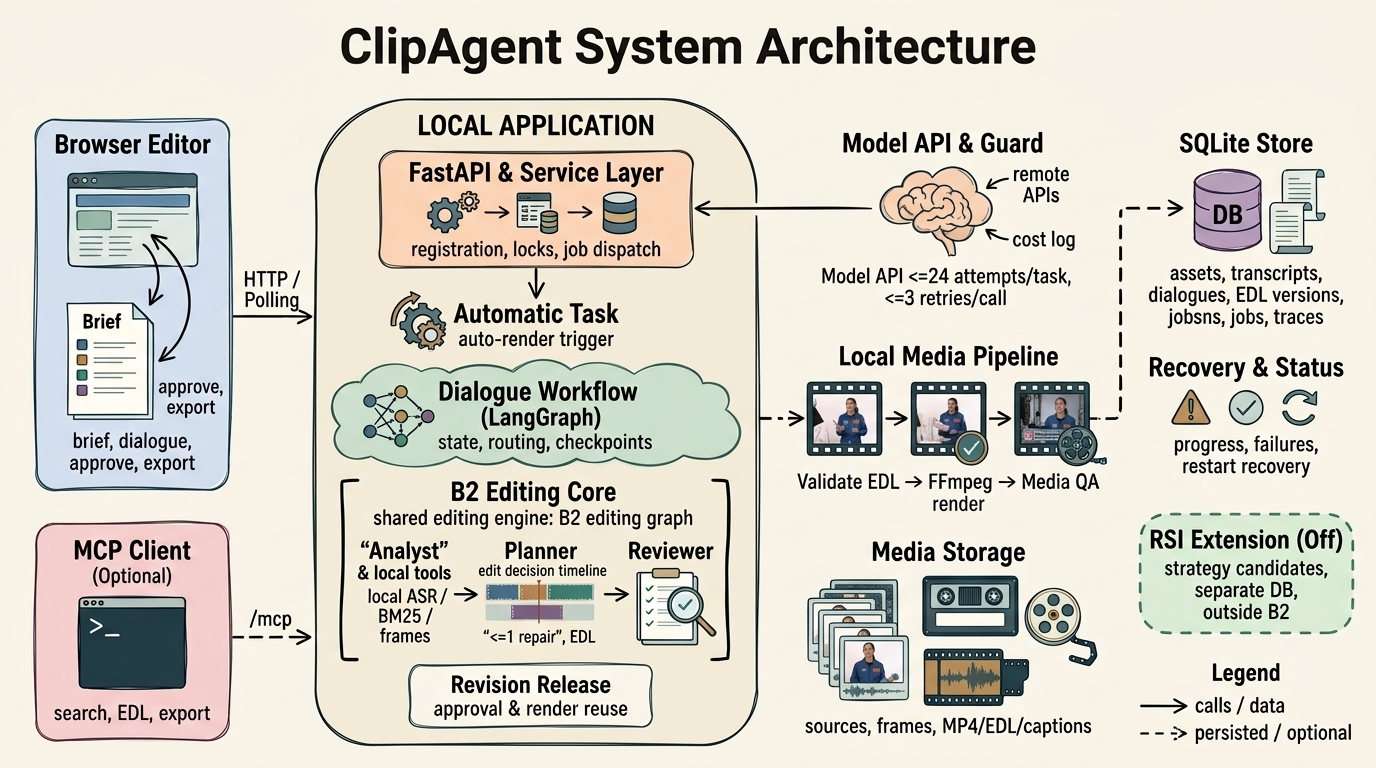
\includegraphics[width=\linewidth,trim=0 0 0 78,clip]{figures/architecture-original.jpeg}}%
\put(807,449){\color{diagramcream}\rule{310\unitlength}{64\unitlength}}%
\put(807,449){\makebox(310,64){\sffamily\fontsize{6.2}{7.4}\selectfont\shortstack{Model API: $\leq 24$ attempts/task\\$\leq 3$ attempts/call (incl. retries)}}}%
\put(1157,430){\color{diagramcream}\rule{199\unitlength}{75\unitlength}}%
\put(1157,430){\makebox(199,75){\sffamily\fontsize{6.0}{7.2}\selectfont\shortstack{Assets, transcripts,\\dialogue, EDL versions,\\jobs and traces}}}%
\end{picture}%
\endgroup%
\caption{ClipAgent system architecture. The local application coordinates dialogue and the shared B2 editing core; remote model calls cross an explicit API boundary, while rendering and media checks run locally. SQLite retains revision and task state. The optional MCP interface and disabled-by-default RSI extension are outside the evaluated B2 configuration. The guard permits at most 24 model HTTP attempts per foreground task and three attempts per call, including retries.}
\label{fig:architecture}
\end{figure}
\paragraph{Preparation and evidence retrieval.}
FastAPI starts and polls asynchronous tasks. Local faster-whisper base \citep{fasterwhisper} transcribes speech with timestamps. BM25 retrieves related transcript spans. An analysis role in LangGraph can read source intervals and inspect sampled frames when the brief requires visual evidence. Local audio processing reduces data sent to remote services. The configured planning and vision endpoints can receive the brief, transcript evidence and sampled frames.

\paragraph{Planning, review, and execution.}
The planning role combines the brief, prior edit, conversation state and tool observations to choose source intervals, order, duration, aspect ratio and subtitle settings. A separate reviewer checks the EDL and can request one repair with a concrete issue. Pydantic schemas and deterministic validators check source bounds, overlap and format constraints. FFmpeg \citep{ffmpeg} executes a validated EDL and checks decoded media, duration, dimensions and subtitle availability. The task record preserves source timecodes and evidence identifiers. Prompts and tool schemas are in \path{app/services/editing_agent.py}, orchestration in \path{app/graph/editing.py}, and rendering in \path{app/services/renderer.py}.


Figure~\ref{fig:workflow} details the editing loop within this architecture. Evidence acquisition supplies timed speech and, when needed, sampled frames. The planner proposes an EDL and the independent reviewer can request at most one semantic repair. A reviewed plan must still pass deterministic validation before FFmpeg renders it; media QA then checks the output. Persisted revision context supports subsequent edits, and approval remains bound to the selected revision rather than to the conversation as a whole.

\begin{figure}[htbp]
\centering
% Remove the artwork's baked-in "Figure 1" heading; numbering belongs to LaTeX.
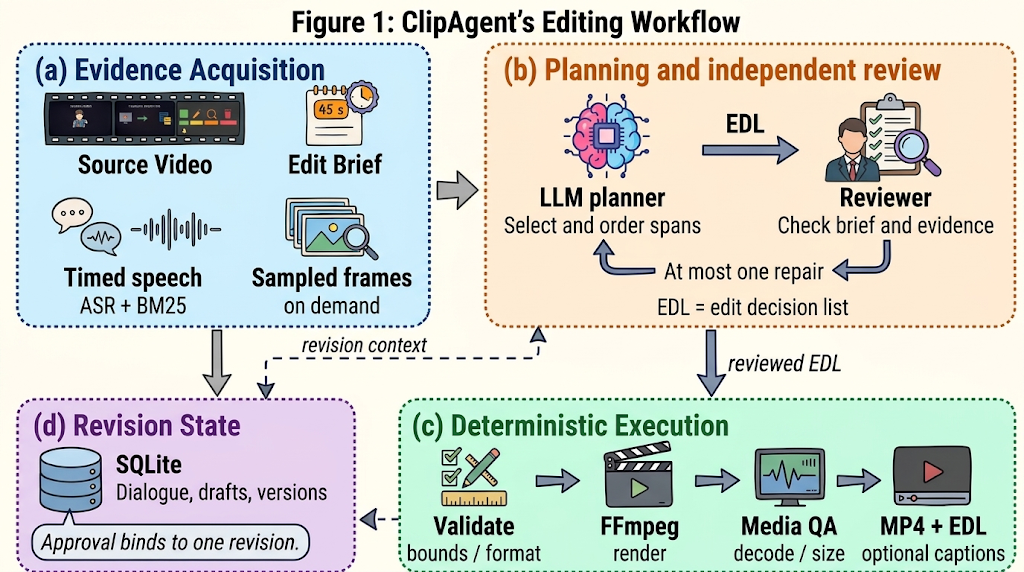
\includegraphics[width=0.88\linewidth,trim=0 0 0 39,clip]{figures/workflow-original.png}
\caption{Evidence-grounded editing workflow. (a) Timed transcript retrieval and on-demand frames ground the brief. (b) The planner selects and orders source spans; an independent reviewer checks the proposal and may request one repair. (c) Deterministic validation, FFmpeg rendering and media QA produce the MP4 and source-linked EDL, with optional captions. (d) SQLite stores dialogue, drafts and versions, providing revision context for follow-up requests.}
\label{fig:workflow}
\end{figure}
\FloatBarrier

\paragraph{State and recovery.}
An explicit requirement overrides prior revision settings and confirmed aspect-ratio or subtitle defaults. SQLite stores drafts, dialogue, tasks and versions. Approval binds to a revision and can reuse a completed render. The isolated restart test restored drafts and downloads, rejected stale approval with HTTP 409, and marked an injected queued task interrupted with a structured error. A missing asset returned HTTP 404. Each foreground task limits model HTTP attempts to 24 across all roles and vision, with at most three attempts per call. Retries count toward this budget because repeated requests can incur additional charges. The UI reports exhausted budgets and failed tasks.

\paragraph{Optional strategy adaptation.}
The RSI module records eligible feedback in a separate database and proposes structured strategy candidates with bounded background work. Offline evaluation and manual activation control which strategies may enter eligible planning prompts. Model weights, tool permissions and validators remain fixed. RSI defaults off and is disabled by the comparison runner. The recorded study predates this module. Automated tests exercise activation, isolation, fallback, and budget exhaustion.

\FloatBarrier
\section{Evaluation protocol}
\label{sec:protocol}
\paragraph{Cases and systems.}
Four explainers each supplied two annotated briefs. The development and held-out splits contain two disjoint sources and four briefs each. The test set covers 30-second vertical explanations and 45-second horizontal recaps, both with English subtitles. Each brief specifies fact units and source reference intervals. B0 takes the opening source window, B1 makes one transcript-based planning call without semantic repair, and B2 runs the full evidence, planning and review workflow. Systems share source preparation and rendering. Applicable duration adjustment is deterministic. We retain the first complete run for each system and brief, including failure cases. The configured text and vision model alias is \texttt{deepseek-flash}. There was no model training or fine-tuning.

\paragraph{Strict scoring.}
The checklist requires all essential facts, faithfulness to the source, no serious cut defect, acceptable subtitles, and correct duration and aspect ratio. Overall strict pass requires all five checks. Two renders failed and remain in the denominator. Gao and Zhang scored the same ten anonymous rendered clips. We preserve each original overall-usable checkbox as a separate measure. When human strict judgments differ, we report the range from confirmed passes to confirmed plus disputed passes.

\paragraph{AI scoring.}
Codex used a fresh faster-whisper transcription of each rendered audio track, sampled frames about every three seconds including the ending, and decoded file measurements. The AI criterion labels and time-coded evidence accompany the submission. The AI had access to parts of the humans' forms and mapping. The AI check is separate and was not strictly blinded. Sampled frames and automatically transcribed speech cannot establish every subtitle cue or speech boundary. AI labels are kept separate from the human decisions.

\section{Results}
\label{sec:results}
\begin{table}[htbp]
\centering
\caption{Frozen runs. Each split contains four assigned briefs per system. Elapsed time is summed after shared asset preparation. Attempts include retries.}
\label{tab:execution}
\begin{tabular}{llrrrr}
\toprule
Split & System & Rendered & Failed & Time (s) & Model attempts \\
\midrule
Development & B0 & 4/4 & 0 & 15.52 & 0 \\
Development & B1 & 0/4 & 4 & 17.42 & 4 \\
Development & B2 & 3/4 & 1 & 300.53 & 85 \\
Test & B0 & 4/4 & 0 & 17.02 & 0 \\
Test & B1 & 2/4 & 2 & 28.48 & 4 \\
Test & B2 & 4/4 & 0 & 268.20 & 81 \\
\bottomrule
\end{tabular}
\end{table}

Table~\ref{tab:execution} shows that B2 completed two more held-out runs than B1 and matched B0's render count. Mean test time per assigned brief was 4.25 seconds for B0, 7.12 for B1, and 67.05 for B2, measured after source preparation and including failed runs. The formal-study usage estimate was USD 0.335423 at the assumed peak uncached rates. The spend guard recorded a USD 2.031448 reservation. Actual provider billing is unconfirmed, and pilot and dialogue work are excluded from the estimate. The AI scoring pass made no paid endpoint calls.

\begin{table}[htbp]
\centering
\caption{Held-out judgments. Strict outcomes use the five criteria jointly. Human bounds include unresolved cases at the upper bound. Stated usability reproduces the original human checkboxes.}
\label{tab:human-ai}
\begin{tabular}{lccccc}
\toprule
System & Gao strict & Zhang strict & Human bounds & AI strict & Gao/Zhang usable \\
\midrule
B0 & 0/4 & 0/4 & 0/4 & 0/4 & 0/4, 0/4 \\
B1 & 1/4 & 1/4 & 1/4 & 0/4 & 2/4, 2/4 \\
B2 & 3/4 & 1/4 & 1/4--3/4 & 1/4 & 4/4, 3/4 \\
\bottomrule
\end{tabular}
\end{table}

Table~\ref{tab:human-ai} reports semantic and editorial quality separately from rendering. Human strict agreement was 8/10 among the renders (Cohen's $\kappa=0.55$). AI agreed with Gao on 7/10 and with Zhang on 9/10. Several clips share the same source, so these are descriptive measures.

\paragraph{Worked cases.}
Clip 03 passed all three checklists. It covered data retrieval, request and response, websites for humans versus APIs for programs, and data endpoint URLs. Clip 05 joined an unfinished suffix-truncation phrase to row versions near 34--37 seconds. Clip 11 retained the restaurant analogy and API definition but had broken joins and a truncated ending. Both remain disputed in the human strict results. Both humans passed clip 09. The AI found a missing endpoint explanation and discontinuities near 10 and 20 seconds. Its EDL contains no source interval past 185.954 seconds, while the annotated endpoint span begins at 194 seconds. A B1 case proposed 47.36 seconds for a 30-second request and stopped at validation. B2 produced a 30.10-second render for that brief, and both humans flagged serious cuts. In a separate development interaction the real model updated an imported plan to a 19.6-second vertical EDL against a 20-second request, retained subtitles and both versions, and used 22 model attempts.

\section{Limitations and broader impacts}
\label{sec:limitations}
Two held-out sources and one execution per brief do not support generalization or statistical significance claims. Sparse frame observations, ASR errors, and subjectivity about cuts and captions all affect judgments. The record separates exact original results from portable replay instructions because provider aliases can change and the project used third-party material. The distribution includes a generated sample, while the source access notes record four hashes and current gaps in third-party attribution and reuse.

Evidence-linked editing can reduce manual search and help educators review clips before sharing. An ill-placed cut can distort meaning or conceal context. Transcripts and visual frames may expose sensitive content to configured services. Traceable intervals, version-specific review, bounded calls, and avoiding credential and source dumps reduce those risks in the prototype.

\section{Contributions and AI disclosure}
\label{sec:disclosure}
Gao Xuefei was the proposal contact and completed independent held-out scoring. Wang Ling coordinated model-service setup and submission. Zhang Yiqun supplied and annotated materials and completed independent held-out scoring. Fu Xuanyu reviewed the reference briefs and intervals. The optional RSI contribution is credited to GitHub author \texttt{phi1220}. The supplied records do not identify which course member owns that account.

The application configures a language model for analysis, planning, and review. Codex assisted with implementation, verification, writing, figure integration and AI assessment. The architecture illustration was supplied as a Gemini-generated image; the workflow illustration was also supplied for this report. Both are explanatory diagrams rather than experimental evidence. Available prompts and omissions are documented in \path{AI_USE.md} and \path{AI_PROMPTS/}. The runnable submission snapshot is \href{https://github.com/Ling-w811/VedioClipAgent/commit/8f5546ec079fd0ee3e90eca954b39178f124f32b}{\texttt{8f5546e}}. The historical study predates the packaging fixes and has separate code and data hashes in \path{evaluation/evidence/freeze.json}.

\begin{thebibliography}{6}
\bibitem{cliptalk} GML-MMGroup. \emph{ClipTalk}. Project repository. \url{https://github.com/GML-MMGroup/ClipTalk}.
\bibitem{videoagent} HKUDS. \emph{VideoAgent}. Project repository. \url{https://github.com/HKUDS/VideoAgent}.
\bibitem{videouse} Browser Use. \emph{video-use}. Project repository. \url{https://github.com/browser-use/video-use}.
\bibitem{openmontage} Calesthio. \emph{OpenMontage}. Project repository. \url{https://github.com/calesthio/OpenMontage}.
\bibitem{fasterwhisper} SYSTRAN. \emph{faster-whisper}. Project repository. \url{https://github.com/SYSTRAN/faster-whisper}.
\bibitem{ffmpeg} FFmpeg Project. \emph{FFmpeg Documentation}. \url{https://ffmpeg.org/documentation.html}.
\end{thebibliography}

\clearpage
\appendix
\section{Item-level decisions and reproducibility}
\label{sec:appendix}

\begin{table}[htbp]
\centering
\caption{The twelve held-out system--brief pairs. Failed executions remain in the overall counts.}
\label{tab:cases}
\begin{tabular}{llccccc}
\toprule
Clip & System & Rendered & Gao strict & Zhang strict & AI strict & Human result \\
\midrule
01 & B0 & Yes & Fail & Fail & Fail & Fail \\
02 & B2 & Yes & Fail & Fail & Fail & Fail \\
03 & B2 & Yes & Pass & Pass & Pass & Pass \\
04 & B1 & No & Fail & Fail & Fail & Fail \\
05 & B2 & Yes & Pass & Fail & Fail & Disputed \\
06 & B1 & Yes & Fail & Fail & Fail & Fail \\
07 & B0 & Yes & Fail & Fail & Fail & Fail \\
08 & B0 & Yes & Fail & Fail & Fail & Fail \\
09 & B1 & Yes & Pass & Pass & Fail & Pass \\
10 & B0 & Yes & Fail & Fail & Fail & Fail \\
11 & B2 & Yes & Pass & Fail & Fail & Disputed \\
12 & B1 & No & Fail & Fail & Fail & Fail \\
\bottomrule
\end{tabular}
\end{table}

\paragraph{Trace pointers.}
Clip 03 corresponds to \texttt{test\_explain\_02\_B} in B2. The EDL trace under \path{evaluation/evidence/test_b2/traces/} records \texttt{read\_video\_content}, \texttt{inspect\_frames}, \texttt{submit\_edit}, and \texttt{submit\_review}. Its span from 198.72 to 210.98 seconds supplies endpoint evidence. The planner, tool definitions and reviewer are connected in \path{app/graph/editing.py}. The failed B1 case \texttt{test\_explain\_01\_A} is in \path{evaluation/evidence/test_b1/results.jsonl}. The restart and missing-source checks have separate verification records.

\paragraph{Package replay.}
The source ZIP includes a standalone browser app, a Windows Python 3.11 lock, generated Nova Cloud source video and prepared captions, a runnable offline B0 case, ordinary/revision/failure requests, and scripts to recompute the recorded scores. The preset has synthetic video with prepared captions. Unit tests can use model stubs. The README run commands exercise these paths without paid credentials. The exact historical videos require approved access through the course-group contact. A historical model rerun also needs a compatible provider credential and an API budget.

\clearpage
\section*{NeurIPS Paper Checklist}




\begin{enumerate}

\item {\bf Claims}
    \item[] Question: Do the main claims made in the abstract and introduction accurately reflect the paper's contributions and scope?
    \item[] Answer: \answerYes{}
    \item[] Justification: Sections~\ref{sec:intro} and~\ref{sec:results} report observed counts and delimit the delivered scope.
    \item[] Guidelines:
    \begin{itemize}
        \item The answer \answerNA{} means that the abstract and introduction do not include the claims made in the paper.
        \item The abstract and/or introduction should clearly state the claims made, including the contributions made in the paper and important assumptions and limitations. A \answerNo{} or \answerNA{} answer to this question will not be perceived well by the reviewers. 
        \item The claims made should match theoretical and experimental results, and reflect how much the results can be expected to generalize to other settings. 
        \item It is fine to include aspirational goals as motivation as long as it is clear that these goals are not attained by the paper. 
    \end{itemize}

\item {\bf Limitations}
    \item[] Question: Does the paper discuss the limitations of the work performed by the authors?
    \item[] Answer: \answerYes{}
    \item[] Justification: Section~\ref{sec:limitations} discusses small sample size, scoring and replay limits.
    \item[] Guidelines:
    \begin{itemize}
        \item The answer \answerNA{} means that the paper has no limitation while the answer \answerNo{} means that the paper has limitations, but those are not discussed in the paper. 
        \item The authors are encouraged to create a separate ``Limitations'' section in their paper.
        \item The paper should point out any strong assumptions and how robust the results are to violations of these assumptions (e.g., independence assumptions, noiseless settings, model well-specification, asymptotic approximations only holding locally). The authors should reflect on how these assumptions might be violated in practice and what the implications would be.
        \item The authors should reflect on the scope of the claims made, e.g., if the approach was only tested on a few datasets or with a few runs. In general, empirical results often depend on implicit assumptions, which should be articulated.
        \item The authors should reflect on the factors that influence the performance of the approach. For example, a facial recognition algorithm may perform poorly when image resolution is low or images are taken in low lighting. Or a speech-to-text system might not be used reliably to provide closed captions for online lectures because it fails to handle technical jargon.
        \item The authors should discuss the computational efficiency of the proposed algorithms and how they scale with dataset size.
        \item If applicable, the authors should discuss possible limitations of their approach to address problems of privacy and fairness.
        \item While the authors might fear that complete honesty about limitations might be used by reviewers as grounds for rejection, a worse outcome might be that reviewers discover limitations that aren't acknowledged in the paper. The authors should use their best judgment and recognize that individual actions in favor of transparency play an important role in developing norms that preserve the integrity of the community. Reviewers will be specifically instructed to not penalize honesty concerning limitations.
    \end{itemize}

\item {\bf Theory assumptions and proofs}
    \item[] Question: For each theoretical result, does the paper provide the full set of assumptions and a complete (and correct) proof?
    \item[] Answer: \answerNA{}
    \item[] Justification: This applied system report presents no theoretical results.
    \item[] Guidelines:
    \begin{itemize}
        \item The answer \answerNA{} means that the paper does not include theoretical results. 
        \item All the theorems, formulas, and proofs in the paper should be numbered and cross-referenced.
        \item All assumptions should be clearly stated or referenced in the statement of any theorems.
        \item The proofs can either appear in the main paper or the supplemental material, but if they appear in the supplemental material, the authors are encouraged to provide a short proof sketch to provide intuition. 
        \item Inversely, any informal proof provided in the core of the paper should be complemented by formal proofs provided in appendix or supplemental material.
        \item Theorems and Lemmas that the proof relies upon should be properly referenced. 
    \end{itemize}

    \item {\bf Experimental result reproducibility}
    \item[] Question: Does the paper fully disclose all the information needed to reproduce the main experimental results of the paper to the extent that it affects the main claims and/or conclusions of the paper (regardless of whether the code and data are provided or not)?
    \item[] Answer: \answerNo{}
    \item[] Justification: Appendix~\ref{sec:appendix} describes runnable code and archived records. The model alias can change and exact source access is restricted.
    \item[] Guidelines:
    \begin{itemize}
        \item The answer \answerNA{} means that the paper does not include experiments.
        \item If the paper includes experiments, a \answerNo{} answer to this question will not be perceived well by the reviewers: Making the paper reproducible is important, regardless of whether the code and data are provided or not.
        \item If the contribution is a dataset and\slash or model, the authors should describe the steps taken to make their results reproducible or verifiable. 
        \item Depending on the contribution, reproducibility can be accomplished in various ways. For example, if the contribution is a novel architecture, describing the architecture fully might suffice, or if the contribution is a specific model and empirical evaluation, it may be necessary to either make it possible for others to replicate the model with the same dataset, or provide access to the model. In general. releasing code and data is often one good way to accomplish this, but reproducibility can also be provided via detailed instructions for how to replicate the results, access to a hosted model (e.g., in the case of a large language model), releasing of a model checkpoint, or other means that are appropriate to the research performed.
        \item While NeurIPS does not require releasing code, the conference does require all submissions to provide some reasonable avenue for reproducibility, which may depend on the nature of the contribution. For example
        \begin{enumerate}
            \item If the contribution is primarily a new algorithm, the paper should make it clear how to reproduce that algorithm.
            \item If the contribution is primarily a new model architecture, the paper should describe the architecture clearly and fully.
            \item If the contribution is a new model (e.g., a large language model), then there should either be a way to access this model for reproducing the results or a way to reproduce the model (e.g., with an open-source dataset or instructions for how to construct the dataset).
            \item We recognize that reproducibility may be tricky in some cases, in which case authors are welcome to describe the particular way they provide for reproducibility. In the case of closed-source models, it may be that access to the model is limited in some way (e.g., to registered users), but it should be possible for other researchers to have some path to reproducing or verifying the results.
        \end{enumerate}
    \end{itemize}


\item {\bf Open access to data and code}
    \item[] Question: Does the paper provide open access to the data and code, with sufficient instructions to faithfully reproduce the main experimental results, as described in supplemental material?
    \item[] Answer: \answerNo{}
    \item[] Justification: Appendix~\ref{sec:appendix} describes the course archive. Third-party MP4s are not openly distributed in it.
    \item[] Guidelines:
    \begin{itemize}
        \item The answer \answerNA{} means that paper does not include experiments requiring code.
        \item Please see the NeurIPS code and data submission guidelines (\url{https://neurips.cc/public/guides/CodeSubmissionPolicy}) for more details.
        \item While we encourage the release of code and data, we understand that this might not be possible, so \answerNo{} is an acceptable answer. Papers cannot be rejected simply for not including code, unless this is central to the contribution (e.g., for a new open-source benchmark).
        \item The instructions should contain the exact command and environment needed to run to reproduce the results. See the NeurIPS code and data submission guidelines (\url{https://neurips.cc/public/guides/CodeSubmissionPolicy}) for more details.
        \item The authors should provide instructions on data access and preparation, including how to access the raw data, preprocessed data, intermediate data, and generated data, etc.
        \item The authors should provide scripts to reproduce all experimental results for the new proposed method and baselines. If only a subset of experiments are reproducible, they should state which ones are omitted from the script and why.
        \item At submission time, to preserve anonymity, the authors should release anonymized versions (if applicable).
        \item Providing as much information as possible in supplemental material (appended to the paper) is recommended, but including URLs to data and code is permitted.
    \end{itemize}


\item {\bf Experimental setting/details}
    \item[] Question: Does the paper specify all the training and test details (e.g., data splits, hyperparameters, how they were chosen, type of optimizer) necessary to understand the results?
    \item[] Answer: \answerYes{}
    \item[] Justification: Section~\ref{sec:protocol} gives the source split, model alias, rubric and system variants. No training was performed.
    \item[] Guidelines:
    \begin{itemize}
        \item The answer \answerNA{} means that the paper does not include experiments.
        \item The experimental setting should be presented in the core of the paper to a level of detail that is necessary to appreciate the results and make sense of them.
        \item The full details can be provided either with the code, in appendix, or as supplemental material.
    \end{itemize}

\item {\bf Experiment statistical significance}
    \item[] Question: Does the paper report error bars suitably and correctly defined or other appropriate information about the statistical significance of the experiments?
    \item[] Answer: \answerNo{}
    \item[] Justification: Section~\ref{sec:limitations} explains why one run per brief on two held-out sources does not support inferential statistics.
    \item[] Guidelines:
    \begin{itemize}
        \item The answer \answerNA{} means that the paper does not include experiments.
        \item The authors should answer \answerYes{} if the results are accompanied by error bars, confidence intervals, or statistical significance tests, at least for the experiments that support the main claims of the paper.
        \item The factors of variability that the error bars are capturing should be clearly stated (for example, train/test split, initialization, random drawing of some parameter, or overall run with given experimental conditions).
        \item The method for calculating the error bars should be explained (closed form formula, call to a library function, bootstrap, etc.)
        \item The assumptions made should be given (e.g., Normally distributed errors).
        \item It should be clear whether the error bar is the standard deviation or the standard error of the mean.
        \item It is OK to report 1-sigma error bars, but one should state it. The authors should preferably report a 2-sigma error bar than state that they have a 96\% CI, if the hypothesis of Normality of errors is not verified.
        \item For asymmetric distributions, the authors should be careful not to show in tables or figures symmetric error bars that would yield results that are out of range (e.g., negative error rates).
        \item If error bars are reported in tables or plots, the authors should explain in the text how they were calculated and reference the corresponding figures or tables in the text.
    \end{itemize}

\item {\bf Experiments compute resources}
    \item[] Question: For each experiment, does the paper provide sufficient information on the computer resources (type of compute workers, memory, time of execution) needed to reproduce the experiments?
    \item[] Answer: \answerNo{}
    \item[] Justification: Section~\ref{sec:results} reports elapsed times and request counts. Exact hosted compute and memory were not available.
    \item[] Guidelines:
    \begin{itemize}
        \item The answer \answerNA{} means that the paper does not include experiments.
        \item The paper should indicate the type of compute workers CPU or GPU, internal cluster, or cloud provider, including relevant memory and storage.
        \item The paper should provide the amount of compute required for each of the individual experimental runs as well as estimate the total compute. 
        \item The paper should disclose whether the full research project required more compute than the experiments reported in the paper (e.g., preliminary or failed experiments that didn't make it into the paper). 
    \end{itemize}
    
\item {\bf Code of ethics}
    \item[] Question: Does the research conducted in the paper conform, in every respect, with the NeurIPS Code of Ethics \url{https://neurips.cc/public/EthicsGuidelines}?
    \item[] Answer: \answerNo{}
    \item[] Justification: The team cannot confirm every third-party reuse term. Section~\ref{sec:limitations} and the archive document this gap.
    \item[] Guidelines:
    \begin{itemize}
        \item The answer \answerNA{} means that the authors have not reviewed the NeurIPS Code of Ethics.
        \item If the authors answer \answerNo, they should explain the special circumstances that require a deviation from the Code of Ethics.
        \item The authors should make sure to preserve anonymity (e.g., if there is a special consideration due to laws or regulations in their jurisdiction).
    \end{itemize}


\item {\bf Broader impacts}
    \item[] Question: Does the paper discuss both potential positive societal impacts and negative societal impacts of the work performed?
    \item[] Answer: \answerYes{}
    \item[] Justification: Section~\ref{sec:limitations} addresses editorial efficiency, misuse through decontextualization, and private source content.
    \item[] Guidelines:
    \begin{itemize}
        \item The answer \answerNA{} means that there is no societal impact of the work performed.
        \item If the authors answer \answerNA{} or \answerNo, they should explain why their work has no societal impact or why the paper does not address societal impact.
        \item Examples of negative societal impacts include potential malicious or unintended uses (e.g., disinformation, generating fake profiles, surveillance), fairness considerations (e.g., deployment of technologies that could make decisions that unfairly impact specific groups), privacy considerations, and security considerations.
        \item The conference expects that many papers will be foundational research and not tied to particular applications, let alone deployments. However, if there is a direct path to any negative applications, the authors should point it out. For example, it is legitimate to point out that an improvement in the quality of generative models could be used to generate Deepfakes for disinformation. On the other hand, it is not needed to point out that a generic algorithm for optimizing neural networks could enable people to train models that generate Deepfakes faster.
        \item The authors should consider possible harms that could arise when the technology is being used as intended and functioning correctly, harms that could arise when the technology is being used as intended but gives incorrect results, and harms following from (intentional or unintentional) misuse of the technology.
        \item If there are negative societal impacts, the authors could also discuss possible mitigation strategies (e.g., gated release of models, providing defenses in addition to attacks, mechanisms for monitoring misuse, mechanisms to monitor how a system learns from feedback over time, improving the efficiency and accessibility of ML).
    \end{itemize}
    
\item {\bf Safeguards}
    \item[] Question: Does the paper describe safeguards that have been put in place for responsible release of data or models that have a high risk for misuse (e.g., pre-trained language models, image generators, or scraped datasets)?
    \item[] Answer: \answerNA{}
    \item[] Justification: The study releases no newly trained models or third-party media collection. Section~\ref{sec:limitations} describes deployment boundaries.
    \item[] Guidelines:
    \begin{itemize}
        \item The answer \answerNA{} means that the paper poses no such risks.
        \item Released models that have a high risk for misuse or dual-use should be released with necessary safeguards to allow for controlled use of the model, for example by requiring that users adhere to usage guidelines or restrictions to access the model or implementing safety filters. 
        \item Datasets that have been scraped from the Internet could pose safety risks. The authors should describe how they avoided releasing unsafe images.
        \item We recognize that providing effective safeguards is challenging, and many papers do not require this, but we encourage authors to take this into account and make a best faith effort.
    \end{itemize}

\item {\bf Licenses for existing assets}
    \item[] Question: Are the creators or original owners of assets (e.g., code, data, models), used in the paper, properly credited and are the license and terms of use explicitly mentioned and properly respected?
    \item[] Answer: \answerNo{}
    \item[] Justification: The archive identifies known source links and records four hashes. Exact provenance and usage terms are incomplete.
    \item[] Guidelines:
    \begin{itemize}
        \item The answer \answerNA{} means that the paper does not use existing assets.
        \item The authors should cite the original paper that produced the code package or dataset.
        \item The authors should state which version of the asset is used and, if possible, include a URL.
        \item The name of the license (e.g., CC-BY 4.0) should be included for each asset.
        \item For scraped data from a particular source (e.g., website), the copyright and terms of service of that source should be provided.
        \item If assets are released, the license, copyright information, and terms of use in the package should be provided. For popular datasets, \url{paperswithcode.com/datasets} has curated licenses for some datasets. Their licensing guide can help determine the license of a dataset.
        \item For existing datasets that are re-packaged, both the original license and the license of the derived asset (if it has changed) should be provided.
        \item If this information is not available online, the authors are encouraged to reach out to the asset's creators.
    \end{itemize}

\item {\bf New assets}
    \item[] Question: Are new assets introduced in the paper well documented and is the documentation provided alongside the assets?
    \item[] Answer: \answerYes{}
    \item[] Justification: Appendix~\ref{sec:appendix} identifies documentation for the application, preset, task manifest and derived scoring records.
    \item[] Guidelines:
    \begin{itemize}
        \item The answer \answerNA{} means that the paper does not release new assets.
        \item Researchers should communicate the details of the dataset\slash code\slash model as part of their submissions via structured templates. This includes details about training, license, limitations, etc. 
        \item The paper should discuss whether and how consent was obtained from people whose asset is used.
        \item At submission time, remember to anonymize your assets (if applicable). You can either create an anonymized URL or include an anonymized zip file.
    \end{itemize}

\item {\bf Crowdsourcing and research with human subjects}
    \item[] Question: For crowdsourcing experiments and research with human subjects, does the paper include the full text of instructions given to participants and screenshots, if applicable, as well as details about compensation (if any)? 
    \item[] Answer: \answerNA{}
    \item[] Justification: The two course-team members judged edited media. The work did not recruit crowd workers or study the raters themselves.
    \item[] Guidelines:
    \begin{itemize}
        \item The answer \answerNA{} means that the paper does not involve crowdsourcing nor research with human subjects.
        \item Including this information in the supplemental material is fine, but if the main contribution of the paper involves human subjects, then as much detail as possible should be included in the main paper. 
        \item According to the NeurIPS Code of Ethics, workers involved in data collection, curation, or other labor should be paid at least the minimum wage in the country of the data collector. 
    \end{itemize}

\item {\bf Institutional review board (IRB) approvals or equivalent for research with human subjects}
    \item[] Question: Does the paper describe potential risks incurred by study participants, whether such risks were disclosed to the subjects, and whether Institutional Review Board (IRB) approvals (or an equivalent approval/review based on the requirements of your country or institution) were obtained?
    \item[] Answer: \answerNA{}
    \item[] Justification: No external participants were recruited or assigned an intervention. Project-member ratings assess the media outputs.
    \item[] Guidelines:
    \begin{itemize}
        \item The answer \answerNA{} means that the paper does not involve crowdsourcing nor research with human subjects.
        \item Depending on the country in which research is conducted, IRB approval (or equivalent) may be required for any human subjects research. If you obtained IRB approval, you should clearly state this in the paper. 
        \item We recognize that the procedures for this may vary significantly between institutions and locations, and we expect authors to adhere to the NeurIPS Code of Ethics and the guidelines for their institution. 
        \item For initial submissions, do not include any information that would break anonymity (if applicable), such as the institution conducting the review.
    \end{itemize}

\item {\bf Declaration of LLM usage}
    \item[] Question: Does the paper describe the usage of LLMs if it is an important, original, or non-standard component of the core methods in this research? Note that if the LLM is used only for writing, editing, or formatting purposes and does \emph{not} impact the core methodology, scientific rigor, or originality of the research, declaration is not required.
    %this research? 
    \item[] Answer: \answerYes{}
    \item[] Justification: Sections~\ref{sec:system}, \ref{sec:protocol} and~\ref{sec:disclosure} describe runtime model use and Codex scoring.
    \item[] Guidelines:
    \begin{itemize}
        \item The answer \answerNA{} means that the core method development in this research does not involve LLMs as any important, original, or non-standard components.
        \item Please refer to our LLM policy in the NeurIPS handbook for what should or should not be described.
    \end{itemize}

\end{enumerate}
\end{document}
